\documentclass[review]{elsarticle}

\usepackage{lineno,hyperref}
\usepackage{color}
\usepackage{amsmath,amsfonts,amssymb,esvect}
\usepackage{float}
\usepackage{graphicx}
\usepackage{epsfig}
%\usepackage{epstopdf}
\usepackage{subcaption}
%\usepackage{subfigure}
\modulolinenumbers[5]

\journal{Journal of \LaTeX\ Templates}


\setlength\parindent{0pt} % Removes all indentation from paragraphs
%\renewcommand{\vec}[1]{\ensuremath{\boldsymbol{#1}}}
\renewcommand{\labelenumi}{\alph{enumi}.} % Make numbering in the enumerate environment by letter rather than number (e.g. section 6)
\newcommand{\px}{\frac{\partial}{\partial x}}
\newcommand{\st}{\sigma_\mathrm{t}}
\newcommand{\pxt}{\frac{\partial^2}{\partial x^2}}
\newcommand{\stt}{\st^2}
\newcommand{\dst}{\frac{\partial\st}{\partial x}}
\newcommand{\pn}{P$_N$}
\newcommand{\pnqt}{P$_N$QT}
\newcommand{\pnqs}{P$_N$QS}
\newcommand{\tp}[1]{TP$_{#1}$}
\newcommand{\ppz}{\frac{\partial}{\partial z}}
\newcommand{\ppzt}{\frac{\partial^2}{\partial z^2}}
\newcommand{\psii}[1]{\psi_\ensuremath{{#1}}}
%%%%%%%%%%%%%%%%%%%%%%%
%% Elsevier bibliography styles
%%%%%%%%%%%%%%%%%%%%%%%
%% To change the style, put a % in front of the second line of the current style and
%% remove the % from the second line of the style you would like to use.
%%%%%%%%%%%%%%%%%%%%%%%

%% Numbered
%\bibliographystyle{model1-num-names}incidation

%% Numbered without titles
%\bibliographystyle{model1a-num-names}

%% Harvard
%\bibliographystyle{model2-names.bst}\biboptions{authoryear}

%% Vancouver numbered
%\usepackage{numcompress}\bibliographystyle{model3-num-names}

%% Vancouver name/year
%\usepackage{numcompress}\bibliographystyle{model4-names}\biboptions{authoryear}

%% APA style
%\bibliographystyle{model5-names}\biboptions{authoryear}

%% AMA style
%\usepackage{numcompress}\bibliographystyle{model6-num-names}

%% `Elsevier LaTeX' style
\bibliographystyle{elsarticle-num}
%%%%%%%%%%%%%%%%%%%%%%%
\newcommand{\zh}{ZrH$_x$}
\newcommand{\e}[1]{\ensuremath{\times 10^{#1}}}
\newcommand{\TAMU}{Texas A\&M University}
\newcommand{\ddxcs}{\sigma(E'\to E,~\mu)}

%\newcommand{\sb1}{\hat{\sigma}_\mathrm{b}}
\begin{document}

\begin{frontmatter}

\title{Accurate Flux-limited Diffusive P$_N$~Closure: P$_N$~Quasi-Transient (P$_N$QT) Model for Radiation Transport}
%\tnotetext[mytitlenote]{Fully documented templates are available in the elsarticle package on \href{http://www.ctan.org/tex-archive/macros/latex/contrib/elsarticle}{CTAN}.}

%% Group authors per affiliation:
\author[mymainaddress]{Weixiong Zheng}
\ead{zwxne2010@tamu.edu}
%% or include affiliations in footnotes:
%\author[mymainaddress,mysecondaryaddress]{Elsevier Inc}
%\ead[url]{www.elsevier.com}

\author[mymainaddress]{Ryan G. McClarren\corref{mycorrespondingauthor}}
\cortext[mycorrespondingauthor]{Corresponding author}
\ead{rgm@tamu.edu}

\address[mymainaddress]{Nuclear Engineering, \TAMU,~College Station, TX 77843-3133}

\begin{abstract}
This template helps you to create a properly formatted \LaTeX\ manuscript.
\end{abstract}

\begin{keyword}
	Flux limited closure\sep Sharp wavefront\sep Spherical harmonics\sep Radiation transport\sep nonlinear
\end{keyword}

\end{frontmatter}

\linenumbers

\section{Introduction}
\subsection{Background and Motivation}

\section{Theories}
\subsection{Cost function deriving P$_N$ equations}
One group transport equation can be given by Eq.~\eqref{te}.
\begin{equation}\label{te}
\frac{1}{v}\frac{\partial\psi(\mathbf{r},\mathbf{\Omega},t)}{\partial t}+\mathbf{\Omega}\cdot\nabla\psi(\mathbf{r},\mathbf{\Omega},t)+\sigma_\mathrm{t}\psi(\mathbf{r},\mathbf{\Omega},t)=q(\mathbf{r},\mathbf{\Omega},t)
\end{equation}

In order to solve it, different angular discretization techniques can be applied. We restrict ourselves on spherical harmonics in the angular treatment.

One could defines the cost function measuring the difference of angular flux, $\psi$~and the spherical harmonics reconstructed angular flux, $\bar{\psi}_N$,~as illustrated Eq.~\eqref{cstf}\cite{mccfpn09}.
\begin{equation}\label{cstf1}
J_1(\mathbf{\Omega})=\int\limits_{4\pi}d\Omega~(\psi-\bar{\psi}_N)^2,
\end{equation}
where
\begin{equation}\label{cstf}
\bar{\psi}_N(\mathbf{\Omega})=\sum_{l=0}^N\sum_{m=-l}^{l}\psi_l^mY^m_l(\mathbf{\Omega}).
\end{equation}
In order to minimize the functional in Eq.~\eqref{cstf},~one force $\partial J_1/\partial\psi_l^m=0$, leading to
the way of computing coefficients of the spherical harmonics expansion, i.e.
\begin{equation}
\psi_l^m=\int\limits_{4\pi}d\Omega\,\psi(\mathbf{\Omega})\bar{Y}_l^m(\mathbf{\Omega}).
\end{equation}

In 1D situation, the expansion degrades to Legendre expansion. The corresponding coefficient is computed by Eq.~\eqref{legendre}.
\begin{equation}\label{legendre}
\psi_l=\int\limits_{-1}^{1}d\mu~\psi(\mu)P_l(\mu)
\end{equation}

Accordingly, take a certain spherical harmonics basis and integrate it with the transport equation over the angular space shall result in corresponding moment equations, e.g. in 1D with isotropic source, the resulting equation is:
\begin{equation}
\frac{1}{v}\partial_t\psi_l+\frac{l}{2l+1}\frac{\partial\psi_{l-1}}{\partial z}(1-\delta_{0,l})+\sigma_{t}\psi_l+\frac{l+1}{2l+1}\frac{\partial\psi_{l+1}}{\partial z}=q_\mathrm{ext}\delta_{0,l},~l=0,1,\cdots
\end{equation}
where $\displaystyle q_\mathrm{ext}=\int\limits_{-1}^1d\mu~q(\mu)$.~In order to close the system truncating at a certain order, N, a convention is to bring in a zero closure at the $(N+1)^\mathrm{th}$~order, i.e.~$\psii{N+1}=0$. Thereafter, the closed \pn~equation system can be described as:
\begin{align}\label{pne}
\frac{1}{v}\partial_t\psi_l+\frac{l}{2l+1}\frac{\partial\psi_{l-1}}{\partial z}(1-\delta_{0,l})+(\sigma_\mathrm{t}-\sigma_\mathrm{s}\delta_{0,l})\psi_l\\\nonumber
+\frac{l+1}{2l+1}\frac{\partial\psi_{l+1}}{\partial z}(1-\delta_{N,l})=q_\mathrm{ext}\delta_{0,l},~l=0,1,\cdots,N.
\end{align}

However, cost function in Eq.~\eqref{cstf1},~rather minimize the square error of \pn~approximated angular flux, it would not necessarily preserve a small residual for \pn~equations.

\subsection{A new cost function in moment space}
\subsubsection{Rewriting \pn~system}
To aid the discussion, we rewrite the \pn~equation such that the closure is separately listed, i.e.
\begin{subequations}
\begin{align}\label{pnmain}
\frac{1}{v}\partial_t\psi_l+\frac{l}{2l+1}\frac{\partial\psi_{l-1}}{\partial z}(1-\delta_{0,l})+(\sigma_\mathrm{t}-\sigma_\mathrm{s}\delta_{0,l})\psi_l\\\nonumber
+\frac{l+1}{2l+1}\frac{\partial\psi_{l+1}}{\partial z}=q_\mathrm{ext}\delta_{0,l},~l=0,1,\cdots,N
\end{align}
\begin{equation}\label{zeroclose}
\psii{N+1}=0,
\end{equation}
\end{subequations}
where the $\delta$~is the Kronecker delta function. The purpose of forming \pn~system in this way is such that we may keep the main body of system along with the paper but only change the closure equation individually.

\subsubsection{A new cost function}
Different from measuring the square error of approximated angular flux, one could also measure the square residual of \pn~approximation as:
\begin{equation}
J(\{\psii{l'}:l'=0,\cdots\})=\int\limits_{-1}^{1}d\mu~R^2,
\end{equation}
where $R$~is the residual. For notation simplicity, we consider the pure absorber problem, leading to the definition of residual as
\begin{align}\label{res}
R\equiv\mathcal{L}\bar{\psi}_N(\mu)-q(\mu)
=\left(\frac{1}{v}\partial_t+\mu\ppz+\st\right)\sum\limits_{l'=0}^{N}\frac{2l'+1}{2}\psii{l'}P_{l'}(\mu)-q(\mu),
\end{align}
where the transport operator $\mathcal{L}$~is defined as:
\begin{equation}
\mathcal{L}\equiv\frac{1}{v}\partial_t+\mu\ppz+\st
\end{equation}

In order to minimize the cost function $J$, we focus on finding moment sets which makes that for all $l$ $\partial J/\partial\psii{l}=0$. Through this path, we could gain an insight into the impact on the residual from the closure.

Taking the function derivative with Eq.~\eqref{res}~leads to:
\begin{align}\label{func}
&\frac{\partial J}{\partial\psii{l}}=(2l+1)\st\int\limits_{-1}^{1}d\mu~RP_l(\mu)+\nonumber\\
(2l+1)\frac{\partial}{\partial\psii{l}}\left[\frac{\partial}{\partial z}\psii{l}\right]&
\int\limits_{-1}^{1}d\mu~R\mu P_l(\mu)+(2l+1)\frac{1}{v}\frac{\partial}{\partial\psii{l}}\left[\frac{\partial}{\partial t}\psii{l}\right]\int\limits_{-1}^{1}d\mu~RP_l(\mu)
\end{align}

Note that for $l\leq N$,~operating the residual with $\displaystyle\int\limits_{-1}^1d\mu~(\cdot)$~results in:
\begin{equation}\label{pnn}
\int\limits_{-1}^1d\mu~RP_l(\mu)=\frac{1}{v}\partial_t\psi_l+\frac{l}{2l+1}\frac{\partial\psi_{l-1}}{\partial z}(1-\delta_{0,l})+\sigma_{t}\psi_l+\frac{l+1}{2l+1}\frac{\partial\psi_{l+1}}{\partial z}-q_\mathrm{ext}\delta_{0,l}.
\end{equation}
Comparing Eq.~\eqref{pnn}~with \pn~equation Eq.~\eqref{pnmain},~one shall see the integral is equal to zero, i.e.
\begin{equation}\label{pnn2}
\int\limits_{-1}^1d\mu~RP_l(\mu)=0,\qquad l\leq N.
\end{equation}

Also, by using recurrence relation of Legendre polynomial, one has:
\begin{equation}\label{recurr}
\int\limits_{-1}^{1}d\mu~R\mu P_l(\mu)=\frac{l}{2l+1}\int\limits_{-1}^{1}d\mu~\mu P_{l-1}(\mu)R+\frac{l+1}{2l+1}\int\limits_{-1}^{1}d\mu~\mu P_{l+1}(\mu)R.
\end{equation}

Therefore, Eq.~\eqref{pnn}~can be rewritten as:
\begin{align}\label{func2}
&\frac{\partial J}{\partial\psii{l}}=(2l+1)\left(\st+\frac{1}{v}\frac{\partial}{\partial\psii{l}}\left[\frac{\partial}{\partial t}\psii{l}\right]\right)\int\limits_{-1}^{1}d\mu~RP_l(\mu)+\nonumber\\
\frac{\partial}{\partial\psii{l}}\left[\frac{\partial}{\partial z}\psii{l}\right]&
\left(l\int\limits_{-1}^{1}d\mu~RP_{l-1}(\mu)+(l+1)\int\limits_{-1}^{1}d\mu~RP_{l+1}(\mu)\right)
\end{align}

Therefore, when $l\leq N-1$,~
plugging Eq.~\eqref{pnn2}~back into Eq.~\eqref{func2}~shall lead to:
\begin{equation}
\frac{\partial J}{\partial\psii{l}}=0.
\end{equation}

So far, we observe the zero-value functional derivative up to Order $N-1$, as expected \textcolor{red}{Shall we talk about our expectation somewhere?}. Nevertheless, we shall be cautious with the same operation when $l=N$,~where the closure lives. 
For $l=N$,~the same substitution, omitting the algebraic process, results in:
\begin{align}\label{func3}
\frac{\partial J}{\partial\psii{N}}=(N+1)
\frac{\partial}{\partial\psii{N}}\left[\frac{\partial}{\partial z}\psii{N}\right]
\left(\int\limits_{-1}^{1}d\mu~RP_{N+1}(\mu)\right).
\end{align}
Therefore, expanding the integral term in Eq.~\eqref{func3}~gives us the final expression for the $N^\mathrm{th}$~order functional derivative:
\begin{align}\label{func4}
\frac{\partial J}{\partial\psii{N}}=&(N+1)
\frac{\partial}{\partial\psii{N}}\left[\frac{\partial}{\partial z}\psii{N}\right]
\left(\frac{1}{v}\partial_t\psi_{N+1}+\frac{N+1}{2N+3}\frac{\partial\psi_{N}}{\partial z}\right.\\\nonumber
&\left.+\sigma_{t}\psi_{N+1}+\frac{N+2}{2N+3}\frac{\partial\psi_{N+2}}{\partial z}\right).
\end{align}

From now on, the discussion for the theoretical part will be mainly based on Eq.~\eqref{func4}~since we realize that it is possible to observe the impacts on residual from the closures through the last functional derivative due to the fact that it contains more than one undetermined moments, which are simply ``thrown away" (zero closure) in conventional \pn~system.

\subsubsection{Discussions on \pn~zero closure}
Introducing zero closure $\psii{\mathcal{M}}=0,~\mathcal{M}>N$ shall result in the following functional derivative:
\begin{equation}\label{bd}
\frac{\partial J}{\partial\psii{N}}=(N+1)
\frac{\partial}{\partial\psii{N}}\left[\frac{\partial}{\partial z}\psii{N}\right]
\frac{N+1}{2N+3}\frac{\partial\psi_{N}}{\partial z}
.
\end{equation}

The treatment of zero closure itself is simple due to the fact that the resulting system is linear and the idea is straightforward. Yet, Eq.~\eqref{bd}~indicates an undesirable property of zero closure: whether or not the minimal residual of \pn~approximation exists depends on the solution itself. 

\subsection{Discussions on diffusive closure}
Levermore et al.~suggested a diffusive closure which takes a form similar to Fick's law for the relationship between $\psii{N+1}$~and $\psii{N}$\cite{levermoredn}:
\begin{equation}\label{fick}
\psii{N+1}=-\frac{1}{\st}\frac{N+1}{2N+3}\ppz\psii{N}
\end{equation}
They, therein, name the corresponding system D$_N$~in the sense that the closure is essentially taking the definition of diffusion on high order moments. Also, Oh and Holloway ~derived a low order D$_2$~method for transient problem by assuming the closed moment $\psii{N+1}$~is time-independent such that one could directly gain the Fick's law like relationship in Eq.~\eqref{fick}\cite{p3qs}.~They name the method P$_3$QS, short for P$_3$~quasi static, because of the gadget used to find the closure. As a extension, we will call diffusive closure method D$_N$ or P$_N$QS at the same time. Since we closed the system at the odd order (i.e.~$N$~is even.), which means the system will have odd numbers of equations differing from conventional \pn,~to keep the system rotationally invariant\textcolor{red}{cite morel's personal talk?}, one shall see D$_{N-1}$~and P$_N$QS are used alternatively in this paper (e.g.~D$_2$~is equivalent to P$_3$QS for time-dependent problems).

Put Eq.~\eqref{fick}~into Eq.~\eqref{func4},~the functional derivative will be turned to be:
\begin{align}\label{bd2}
\frac{\partial J}{\partial\psii{N}}=&(N+1)
\frac{\partial}{\partial\psii{N}}\left[\frac{\partial}{\partial z}\psii{N}\right]
\left(\frac{1}{v}\partial_t\psi_{N+1}+\frac{N+2}{2N+3}\frac{\partial\psi_{N+2}}{\partial z}\right).
\end{align}

Though the way of deriving P$_N$QS method is to assume the closure to be time-independent, the independency is only weakly imposed. The assumption transfer the time-dependency of closure moment, $\psii{N+1}$, to that of $\psii{N}$.~This can be seen by simply plug Eq.~\eqref{fick}~back in \eqref{bd2}:
\begin{equation}
\frac{\partial J}{\partial\psii{N}}=(N+1)
\frac{\partial}{\partial\psii{N}}\left[\frac{\partial}{\partial z}\psii{N}\right]
\left(-\frac{N+2}{2N+3}\frac{1}{v}\partial_t\left(\frac{1}{\st}\ppz\psii{N}\right)+\frac{N+2}{2N+3}\frac{\partial\psi_{N+2}}{\partial z}\right).
\end{equation}

The result in Eq.~\eqref{bd2}~is interesting in several aspects: one on hand, it still preserves the solution dependency of the functional derivative, which means the closure would lead to small residual only if the solution holds high regularity in time and space; on the other hand, the derivative includes a temporal derivative of the solution, which means the functional derivative could be small when the solution varies slowly in time. The first point illustrates the why numerical results are away from exact solution in some test problems; meanwhile, the second point might indicate when the short transient passed, $\partial_t(\cdot)\sim 0$,~the solution is relatively accurate.
\subsection{Two new nonlinear closures}
\subsubsection{Approximations on higher moments}
Eq.~\eqref{func4},~in some senses, theoretically indicates if one could find a closure such that:
\begin{equation}\label{func5}
\frac{1}{v}\partial_t\psi_{N+1}+\frac{N+1}{2N+3}\frac{\partial\psi_{N}}{\partial z}
+\sigma_{t}\psi_{N+1}+\frac{N+2}{2N+3}\frac{\partial\psi_{N+2}}{\partial z}=0,
\end{equation}
which is equivalent to introduce higher order \pn~approximation without changing the truncation order, the closure, leading to zero functional derivative in moment space, would potentially leads to minimum residual of the \pn~approximation. However, this is feasible practically since truncating at a certain order $N$~would lead to the loss of information of high orders, e.g.~$\psii{N+2}$. The value of Eq.~\eqref{func5}~is that it implies one would find a proper way to approximate high orders to minimize the residual in moment space.

Rewrite Eq.~\eqref{func5},~the closure can be expressed as a transcendental functional:
\begin{equation}\label{oricl}
\psii{N+1}=-\frac{1}{\sigma_\mathrm{t}+\displaystyle\frac{1}{v\psii{N+1}}\partial_t\psii{N+1}+\frac{(N+2)}{(2N+3)\psii{N+1}}\ppz\psii{N+2}}\frac{N+1}{2N+3}\ppz\psii{N}
\end{equation}
It basically preserves the form of diffusive closure, yet, the derivatives on sides of $\st$~are like adjustments to the cross sections.

In order to make the system closed, one potential way is to mimic the undetermined moments using moments within the truncation order. If one assumes that the angular flux is separable in time in the following way:
\begin{equation}\label{sep1}
\psi(z,\mu,t)=T(t)\hat{\phi}(\mu,z)+r_t(z,\mu,t),
\end{equation}
where the $r_t(z,\mu,t)$~is the rest part of the separation, and the separated part is dominant, one could find:
\begin{equation}
\frac{1}{v\psii{N+1}}\partial_t\psii{N+1}\sim\frac{1}{v\psii{0}}\partial_t\psii{0}.
\end{equation}
Meanwhile, if one could assume:
\begin{equation}\label{sep2}
\psi(z,\mu,t)=\phi(z)\hat{U}(\mu,t)+r_z(z,\mu,t),
\end{equation}
where the $r_z(z,\mu,t)$~is the rest part of the separation, and the separated part is dominant, one could find:
\begin{equation}
\frac{(N+2)}{(2N+3)\psii{N+1}}\ppz\psii{N+2}\sim\alpha(i,j,\hat{U})\frac{\partial_z\psii{i}}{\psii{j}},
\end{equation}
where
\begin{equation}
\alpha(i,j,\hat{U})=\frac{(N+2)\displaystyle\int\limits_{-1}^1d\mu~P_{N+2}(\mu)\hat{U}(\mu,t)\cdot\int\limits_{-1}^1d\mu~P_{j}(\mu)\hat{U}(\mu,t)}{(2N+3)\displaystyle\int\limits_{-1}^1d\mu~P_{N+1}(\mu)\hat{U}(\mu,t)\cdot\int\limits_{-1}^1d\mu~P_{i}(\mu)\hat{U}(\mu,t)}.
\end{equation}
Hence, the resulting closure could be given by:
\begin{equation}\label{closure}
\psii{N+1}=-\frac{1}{\sigma_\mathrm{t}+\displaystyle\frac{1}{v\psii{0}}\partial_t\psii{0}+\frac{\alpha(i,j,,\hat{U})\partial_z\psii{i}}{\psii{j}}}\frac{N+1}{2N+3}\ppz\psii{N}
\end{equation}
To preserve the positivity of ``adjusted cross section", the denominator, we chose to use:
\begin{equation}\label{closure2}
\psii{N+1}=-\frac{1}{\sigma_\mathrm{t}+\displaystyle|\frac{1}{v\psii{0}}\partial_t\psii{0}|+|\frac{\alpha(i,j,\hat{U})\partial_z\psii{i}}{\psii{j}}|}\frac{N+1}{2N+3}\ppz\psii{N}
\end{equation}

Yet, we still need to do some compromise on $\alpha$~to make the closure function well. The $\alpha$,~if it is archivable, it would depend on the angular distribution of the flux besides the order pair $(i,j)$~one chooses. A simple modification is that one choose a constant $\alpha$~for a specific $(i,j)$. All these approximations, though does not guarantee the minimum residual, does add potentially proper modification on diffusivity of the closure to the diffusive closure.

\subsubsection{A moment-limited closure}
Specifically, (0,N)~is of interest due to one of properties demonstrated below. With this order pair, the closure function is:
\begin{equation}
\psi_{N+1}=\frac{1}{\sigma_\mathrm{t}+\displaystyle|\frac{\partial_t\psii{0}}{v\psii{0}}|+\alpha|\frac{\partial_z\psii{N}}{\psii{0}}|}\frac{N+1}{2N+3}\ppz\psii{N}
\end{equation}

If one chooses the pair $(0,N)$~and carefully pick an $\alpha$, one could prove that this setting limits the magnitudes of the closure as follows:
\begin{align}
|\psi_{N+1}|=\frac{1}{\sigma_\mathrm{t}+\displaystyle|\frac{\partial_t\psii{0}}{v\psii{0}}|+\alpha|\frac{\partial_z\psii{N}}{\psii{0}}|}\frac{N+1}{2N+3}|\ppz\psii{N}|\\\nonumber
<\frac{1}{\displaystyle\alpha|\frac{\partial_z\psii{N}}{\psii{0}}|}\frac{N+1}{2N+3}|\ppz\psii{N}|=\frac{N+1}{\alpha(2N+3)}|\psi_0|
\end{align}

For instance, fixing $\alpha$~at $(N+1)/(2N+3)$~would result in:
\begin{equation}
|\psii{N+1}|<|\psii{0}|
\end{equation}

That is similar to the situation of limiting current to the scalar flux (energy) to stabilize the system in moment space. We, therefore, name the closure moment-limited diffusive closure.

\subsubsection{A modification: flux-limited closure}
Another simple choice of (i,j)~is (0,0)~leading to the fact that the closure is similar to Larsen-type flux limiter (with $n=1$) used in flux limited diffusion (\textcolor{red}{cit larsen sth}). In this sense, this closure is a high order extension of flux-limited diffusion with an additional constraint from temporal evolution of flux (i.e. the $\partial_t\psii{0}$~term). Specifically, the closure is expressed as:

\begin{equation}\label{closure3}
\psii{N+1}=-\frac{1}{\sigma_\mathrm{t}+\displaystyle|\frac{1}{v\psii{0}}\partial_t\psii{0}|+|\frac{\alpha(0,0,\hat{U})\partial_z\psii{0}}{\psii{0}}|}\frac{N+1}{2N+3}\ppz\psii{N}
\end{equation}

Since we perform similar (but not identical) operational on the closed moment as Larsen-type flux limited diffusion, we name the closure flux-limited diffusive closure. $\alpha$~depends on the angular flux distribution making computing it complex and nonlinear. For simplicity,
we, instead, fix the $\alpha$~in Eq.~\eqref{closure3}~to a constant as same as moment-limited closure. A simple choice working well is to choose a number from the Jacobian of \pn~system.

The central theme is the similar to the moment-limited closure that one adjusts the diffusivity nonlinearly based on the solution. The difference is that the adjustment is done by watching on scalar flux only without taking any other high moment into account. It is hard to realize the limitation it puts on the closure in analytic form. Nevertheless, it is possible to analyze that qualitatively.

Assuming forward Euler time discretization is performed such that the closure is evolved using the previous moment information. In a semi-discrete scheme, the closure at time Step 1 will be formulated as:
\begin{equation}\label{closuresemi1}
\psii{N+1}^{(1)}=-\frac{1}{\sigma_\mathrm{t}+\displaystyle|\frac{1}{v\psii{0}^{(0)}}\partial_t\psii{0}^{(0)}|+|\frac{\alpha\partial_z\psii{0}^{(0)}}{\psii{0}^{(0)}}|}\frac{N+1}{2N+3}\ppz\psii{N}^{(0)}
\end{equation}
If the initial condition holds that the angular flux is isotropic (also true for zero flux scenario), which is true for the problems tested in this paper, it is true the claim that $\exists$~finite number $\beta>0$~such that $\psii{0}^{(0)}\geq\beta\psii{N}^{(0)}$. In isotropic-flux initial condition, $\psii{N}^{(0)}=0$, thus the claim is always true with $\beta=1$.

Introducing the inequality to Eq.~\eqref{closuresemi1},~and take the absolute values, one shall see the following limitation on the closure at first time step:
\begin{align}\label{closuresemi2}
&|\psii{N+1}^{(1)}|<\frac{1}{\sigma_\mathrm{t}+\displaystyle|\frac{1}{v\psii{0}^{(0)}}\partial_t\psii{0}^{(0)}|+|\frac{\alpha\partial_z\psii{0}^{(0)}}{\psii{0}^{(0)}}|}\frac{N+1}{2N+3}|\ppz\psii{N}^{(0)}|\\\nonumber
&<\frac{1}{\displaystyle|\frac{\alpha\partial_z\psii{0}^{(0)}}{\psii{0}^{(0)}}|}\frac{N+1}{2N+3}|\ppz\psii{N}^{(0)}|\leq\frac{1}{\displaystyle|\frac{\alpha\partial_z\left(\beta^{(0)}\psii{N}^{(0)}\right)}{\psii{0}^{(0)}}|}\frac{N+1}{2N+3}\lvert\ppz\psii{N}^{(0)}\rvert\\\nonumber
&=\frac{N+1}{\alpha\beta^{(0)}(2N+3)}|\psii{0}^{(0)}|
\end{align}

Qualitatively, at the first time step, Eq.~\eqref{closuresemi2}~is true if and only if the angular flux is bounded by some finite value $\mathcal{B}$ (it is realizable that unbounded angular flux would cause large variations in moment space),~i.e.~$|\psi(\mu)^{(1)}|\leq\mathcal{B}^{(1)}$, so reversely, it tells us every other moment must be bounded. Somehow, this is equivalent to give the relationship between $\psii{N}$~and $\psii{0}$~at the first time step: $\exists$~a finite number $\beta^{(1)}$, such that
\begin{equation}
\lvert\psii{N}^{(1)}\rvert\leq\beta^{(1)}|\psii{0}^{(1)}|,
\end{equation}
leading to:
\begin{equation}
|\psii{N+1}^{(2)}|<\frac{N+1}{\alpha\beta^{(2)}(2N+3)}|\psii{0}^{(1)}|
\end{equation}
Similarly, one could use induction to qualitatively demonstrate that, there is always a finite number $\beta^{(n+1)}$~at Step $n+1$, such that
\begin{equation}
|\psii{N+1}^{(n+1)}|<\frac{N+1}{\alpha\beta^{(n+1)}(2N+3)}|\psii{0}^{(n)}|
\end{equation}
Take the limit of zero for the time step length $\delta t$,~the discrete inequality is turned to be continuous in time, i.e.~at a certain time $t$, $\exists~0<\beta(t)<\infty$~such that:
\begin{equation}\label{fld}
|\psii{N+1}(t)|<\frac{N+1}{\alpha\beta(t)(2N+3)}|\psii{0}(t)|
\end{equation}

In summary, both the moment-limited and flux-limited diffusive closure are to try to suppress unphysical information flow in $\psii{N+1}$~and bound it by the scalar flux. All the limiting efforts eventually result in the simulated flux profile closely twirling around the exact solution and effectively dampening the unphysical modes (large spikes), which leads to relatively accurate solutions for the transport problem in short-time transient. In this sense, we name the closure model P$_N$~quasi transient model (P$_N$QT). 

\section{Semi-discrete solution schemes and boundary condition consistency}
Denote the moment set $\{\psii{0},\cdots,\psii{N+1}\}$~by a column vector $\vec{\phi}$ and let $\vec{Q}=\left(q_\mathrm{ext},0,\cdots,0\right)^T$,~then the system can be rewritten as:
\begin{subequations}
	\begin{equation}
	\frac{1}{v}\partial_t\vec{\phi}+\ppz\left(\mathbf{A}\vec{\phi}\right)+\mathbf{\Sigma}\vec{\phi}=\vec{Q}
	\end{equation}
	\begin{equation}
	\psi_{N+1}=\frac{1}{\sigma_\mathrm{t}+\displaystyle|\frac{\partial_t\psii{0}}{v\psii{0}}|+\alpha|\frac{\partial_z\psii{j}}{\psii{0}}|}\frac{N+1}{2N+3}\ppz\psii{N},
	\end{equation}
\end{subequations}
where the $\mathbf{A}$~is the Jacobian matrix containing the coefficients of the derivative terms and $\mathbf{\Sigma}$~is a diagonal matrix with the form (assuming isotropic scattering):
\begin{equation}
\mathbf{\Sigma}=\mathrm{diag}\{\sigma_\mathrm{a},\sigma_\mathrm{t},\cdots,\sigma_\mathrm{t}\}
\end{equation}

\subsection{Time stepping}
We forward the information for moments using backward Euler. However, fully-implicit treatment on the closure would largely increase the computational cost. Alternatively, while keeping using implicit scheme on the moments, the limiters are evolved explicitly, then the system could be differenced in time as:
\begin{subequations}
	\begin{equation}
	\frac{1}{v\Delta t}\vec{\phi}^{~(n+1)}+\ppz\left(\mathbf{A}\vec{\phi}\right)^{(n+1)}+\mathbf{\Sigma}\vec{\phi}^{~(n+1)}=\vec{Q}^{~(n+1)}+\frac{1}{v\Delta t}\vec{\phi}^{~(n)}
	\end{equation}
	\begin{align}\label{closuresemin}
	\psii{N+1}^{(n+1)}=-\frac{1}{\sigma_\mathrm{t}+\displaystyle|\frac{\psii{0}^{(n)}-\psii{0}^{(n-1)}}{v\Delta t\psii{0}^{(n)}}|+|\frac{\alpha\partial_z\psii{j}^{(n)}}{\psii{0}^{(n)}}|}\frac{N+1}{2N+3}\ppz\psii{N}^{(n+1)},
	\end{align}
\end{subequations}
where $j=0$(flux limiter) or $j=N$(moment limiter). Once the time step is small enough, the lags on evaluating limiters could be negligible and the scheme is then justified.

To start the time stepping for $t=0$,~we simply used diffusive closure,~without any limiter, for the first two time steps.

\subsection{Spatial discretization}
Spatially, diamond difference (DD) is performed. Therefore, all the moments live on the nodes. The semi-discrete scheme is shown below:
\begin{subequations}
	\begin{equation}
	\frac{1}{v}\partial_t\vec{\phi}^{~i}+\mathbf{A}\frac{\left(\vec{\phi}^{~i+1/2}-\vec{\phi}^{~i-1/2}\right)}{\Delta z}+\mathbf{\Sigma}^{~i}\vec{\phi}^{~i}=\vec{Q}^{~i}
	\end{equation}
	\begin{equation}
	\psi_{N+1}^{~i}=\frac{1}{\sigma_\mathrm{t}^i+\displaystyle|\frac{\partial_t\psii{0}^{~i}}{v\psii{0}^{~i}}|+\alpha|\frac{\psii{j}^{~i+1/2}-\psii{j}^{~i-1/2}}{\Delta z\psii{0}^{~i}}|}\frac{N+1}{2N+3}\frac{\psii{N}^{~i+1/2}-\psii{N}^{~i-1/2}}{\Delta z},
	\end{equation}
	\begin{equation}
	(\cdot)^i=\frac{(\cdot)^{~i+1/2}+(\cdot)^{~i-1/2}}{2}
	\end{equation}
\end{subequations}
where $i=1,\cdots,I$~denotes the cell numbers.

\subsection{Boundary condition consistency}
Another option of solving the system is to substitute the closure moment in $\vec{\phi}$~with the Fick's-law like expression and solve a mix-order system. This would bring computational advantage that if one close the system at even order \pn~approximation, the number of unknowns will be reduced, especially in multi-D application, e.g. in Holloway's work, the P$_3$QS (D$_2$) has six unknowns instead of ten unknowns of P$_3$~approximations.

However, one shall be cautious on the boundary treatment. When invoking half-range integrations of the moments (either Marshak or Mark boundary methodology), the highest order of mix-order form is even. A natural thought take $N/2$ half integrals with odd order Legendre polynomial and one integral with even order Legendre polynomial on one side of the slab. We shall see in Section~\ref{num}~that in applications with incident boundary conditions the flux profile will have unphysical discrepancy with the real solution.

Instead, we used conventional treatment that integrating with odd order Legendre polynomials up to $N+1$ (recall we close the system at even orders, e.g. $N=2$, so we would not have $\psii{3}$ in mix-order formulation). Consistently, we need to approximate the $\psii{N+1}$~with the closure on the boundary. For instance, when closing the system at $\psii{2}$,~the Marshak boundary condition on the left side of the domain could be expressed as:
\begin{equation}
\int\limits_{\mu>0}d\mu~\psi_{\mathrm{inc}}(\mu)P_l(\mu)=\sum\limits_{i=0}^{2}c_i\psii{i}-c_3\frac{1}{\sigma_\mathrm{t}+\displaystyle|\frac{\partial_t\psii{0}}{v\psii{0}}|+\alpha|\frac{\partial_z\psii{j}}{\psii{0}}|}\frac{3}{7}\ppz\psii{2},
\end{equation}
where $l=1,3$~and $\displaystyle c_i=\int_{\mu>0}d\mu~P_l(\mu)P_i(\mu)$.~The treatment above introduces nonlinearity on boundary, though, it would not take much extra work if the limiters are forwarded explicitly in time consistent with Eq.~\eqref{closuresemin}.

\section{Numerical results}\label{num}
\subsection{Plane source problem: capturing short-time transient}
The first test problem is the 1D slab plane source problem. The medium is a pure scatterer ($\st=1,~\sigma_\mathrm{s}=1$).~At time $t=0$,~there is a pulse in the middle of the slab and afterwards the particles spread out in the pure scattering medium. The initial condition could be described as:
\begin{equation}
\psi(z,\mu,0)=\frac{\delta(z)}{2}
\end{equation}
The boundary condition is simply to vanish the angular flux at infinitely far place, i.e.
\begin{equation}
\psi(\pm\infty,\mu,t)=0.
\end{equation}
This test is featured by a step wavefront at $z=\pm vt$,~which stimulates \pn~approximation to generate unphysical solutions when trying to fit the wavefront. In fact, this keeps particles staying in peaks at $\pm\lambda_ivt$~and waiting for collisions. The consequence is, the solutions will have $N+1$~spikes,~mathematically depicted by Dirac delta function, for a long time. In the following part the numerical solutions will be compared with the analytic transport solution from the benchmark suite AZURV1\cite{ganapol}.

\subsubsection*{Comparison with \pn~approximation}
In the short-time transients, flux magnitudes around $z=\pm vt$~are unphysically high while the flux is over-suppressed anywhere else. Increasing the order of \pn~does not help fix the over-suppression much. 

In contrast, P$_N$QT model effectively weakens the artificial discontinuities in the solutions. At the same time, the over-suppression is somehow recovered.

\begin{figure}[ht!]
	\begin{center}
		\hspace*{-3cm}\includegraphics[width=1.4\textwidth]{vspnt1p0.eps}
		%\includegraphics[width=0.45\textwidth]{srholam.eps}
		\caption[]{\label{pn1p0}Planar source problem: comparison of scalar flux with \pn,~t=1s.}% Only the ``Figure" label and figure number are bold.}
	\end{center}
\end{figure}

\begin{figure}[ht!]
	\begin{center}
		\hspace*{-3cm}\includegraphics[width=1.4\textwidth]{vspnt3p0.eps}
		%\includegraphics[width=0.45\textwidth]{srholam.eps}
		\caption[]{\label{pn3p0}Planar source problem: comparison of scalar flux with \pn,~t=3s.}% Only the ``Figure" label and figure number are bold.}
	\end{center}
\end{figure}

\begin{figure}[ht!]
	\begin{center}
		\hspace*{-3cm}\includegraphics[width=1.4\textwidth]{vspnt5p0.eps}
		%\includegraphics[width=0.45\textwidth]{srholam.eps}
		\caption[]{\label{pn5p0}Planar source problem: comparison of scalar flux with \pn,~t=5s.}% Only the ``Figure" label and figure number are bold.}
	\end{center}
\end{figure}

\subsubsection*{Comparison with P$_N$QS (D$_{N-1}$)~approximation}
In order to make the boundary conditions fit the system, we close the systems at even order moments, e.g.~plugging the closure equation for P$_3$QT back into the main system results in a system with $\psii{2}$~as the highest-order moment. The diffusive closure (D$_N$)~is equivalent to introduce sort of physics based viscosity in the highest moment equation. The closure is with the form of Fick's law. In steady state problems, where the time-dependent term is gone, D$_{N-1}$~is essentially P$_N$ approximation. P$_N$QT is, based on the diffusive closure, to put a constraint on the spatial and temporal variations of moments(moment limited) or flux (flux limited). The origin is to fix the fact that diffusive closure does not force any boundedness of the moments. So there is still possibilities that moments go beyond the flux causing unphysical solutions in time dependent problems with short-time transient.

Due to facts above, we compare the even order \pn~with \pnqs~and \pnqt~in Figure~\ref{epn}~and \ref{epn2}.

\begin{figure}[ht!]
	\begin{center}
		\hspace*{-0cm}\includegraphics[width=1.\textwidth]{vsp2.eps}
		%\includegraphics[width=0.45\textwidth]{srholam.eps}
		\caption[]{\label{epn}Planar source problem: comparisons among P$_2$,~P$_3$QS,~P$_3$QT,~t=0.5s.}% Only the ``Figure" label and figure number are bold.}
	\end{center}
\end{figure}

\begin{figure}[ht!]
	\begin{center}
		\hspace*{-0cm}\includegraphics[width=1.\textwidth]{vsp4.eps}
		%\includegraphics[width=0.45\textwidth]{srholam.eps}
		\caption[]{\label{epn2}Planar source problem: comparisons among P$_4$,~P$_5$QS,~P$_5$QT,~t=0.5s.}% Only the ``Figure" label and figure number are bold.}
	\end{center}
\end{figure}

In Figure~\ref{epn},~we present the comparison among P$_2$,~P$_3$QS (D$_2$)~and P$_3$QT. The stationary mode of even order \pn~decays slowly. The diffusive closure, however, removes the stationary mode. However, it simultaneously slows down the speed of the moving mode, which consequently slows down the process of converging to the real transport solution in time. Furthermore, the dissipation added to the stationary mode over-suppresses the scalar flux and actually transfer the particles to the moving mode making D$_2$~have high magnitudes.

P$_3$QT, yet, automatically adjusted the dissipation added to the main mode in the middle. And it spread the particles around the static mode instead of transfering them into the moving modes so that flux limited closure has accurate values in the middle of the domain without lots of uncollided particles staying in the moving modes waiting for collisions. And also the P$_3$QT, somehow, fixes the slowing down of the mode speed and recovers it close to P$_2$ mode speed.

Similar phenomena occur to higher order approximations (Figure~\ref{epn2}~presents example for P$_4$.)\textcolor{red}{I think we 'd better use P6 to show a ``high" order approximation}, indicating the dissipation behavior of the stationary of all closures generally exists in even order \pn~methodology.

\begin{figure}[ht!]
	\begin{center}
		\hspace*{-3cm}\includegraphics[width=1.4\textwidth]{vsdnt0p5.eps}
		%\includegraphics[width=0.45\textwidth]{srholam.eps}
		\caption[]{\label{dn0p5}Planar source problem: comparison of scalar flux with P$_N$QS (D$_{N-1}$),~t=0.5s.}% Only the ``Figure" label and figure number are bold.}
	\end{center}
\end{figure}

\begin{figure}[ht!]
	\begin{center}
		\hspace*{-3cm}\includegraphics[width=1.4\textwidth]{vsdnt2p0.eps}
		%\includegraphics[width=0.45\textwidth]{srholam.eps}
		\caption[]{\label{dn2p0}Planar source problem: comparison of scalar flux with P$_N$QS (D$_{N-1}$),~t=2s.}% Only the ``Figure" label and figure number are bold.}
	\end{center}
\end{figure}

\begin{figure}[ht!]
	\begin{center}
		\hspace*{-3cm}\includegraphics[width=1.4\textwidth]{vsdnt4p0.eps}
		%\includegraphics[width=0.45\textwidth]{srholam.eps}
		\caption[]{\label{dn4p0}Planar source problem: comparison of scalar flux with P$_N$QS (D$_{N-1}$),~t=4s.}% Only the ``Figure" label and figure number are bold.}
	\end{center}
\end{figure}

We also compare P$_N$QT with \pnqs~at several time points (Figure~\ref{dn0p5},~\ref{dn2p0}~and \ref{dn4p0}),~the fixation of over-suppression from \pnqt~is significant. In addition, with accelerating the moving modes, the \pnqt~converge to the transport solution much faster than the diffusive closure.
%The slab is infinitely long. The boundary condition is vacuum boundary condition.
%
%With time flying by, the particles collide. But there is always a step-function like wavefront at $z=vt$ (\textcolor{red}{is ti a step function here from Ganpol's work?}). This discontinuity in the solution drives conventional \pn~method crazy on resolving it with finite Legendre expansion. Particles  stays in the eigen-modes and never collides resulting in spikes in the solution (theoretically, they are depicted by Dirac delta functions).



\subsection{Double incidents problem}

\begin{figure}[ht!]
	\begin{subfigure}{.9\textwidth}
		\centering
		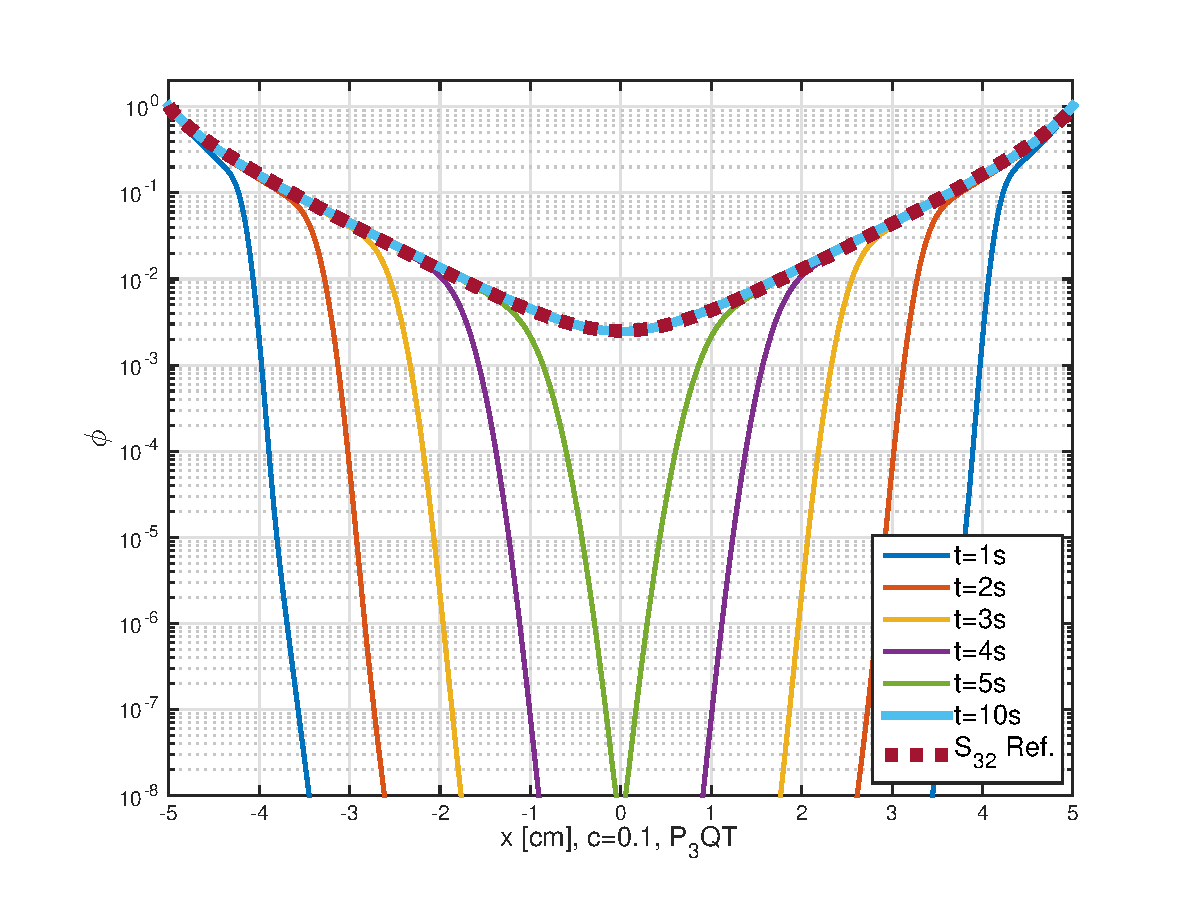
\includegraphics[width=1\linewidth]{brunner_p3qt.eps}
		%\caption{P$_3$QT time-dependent solution}
		%\label{bmtrhort}
	\end{subfigure}
	~
	\begin{subfigure}{.9\textwidth}
		\centering
		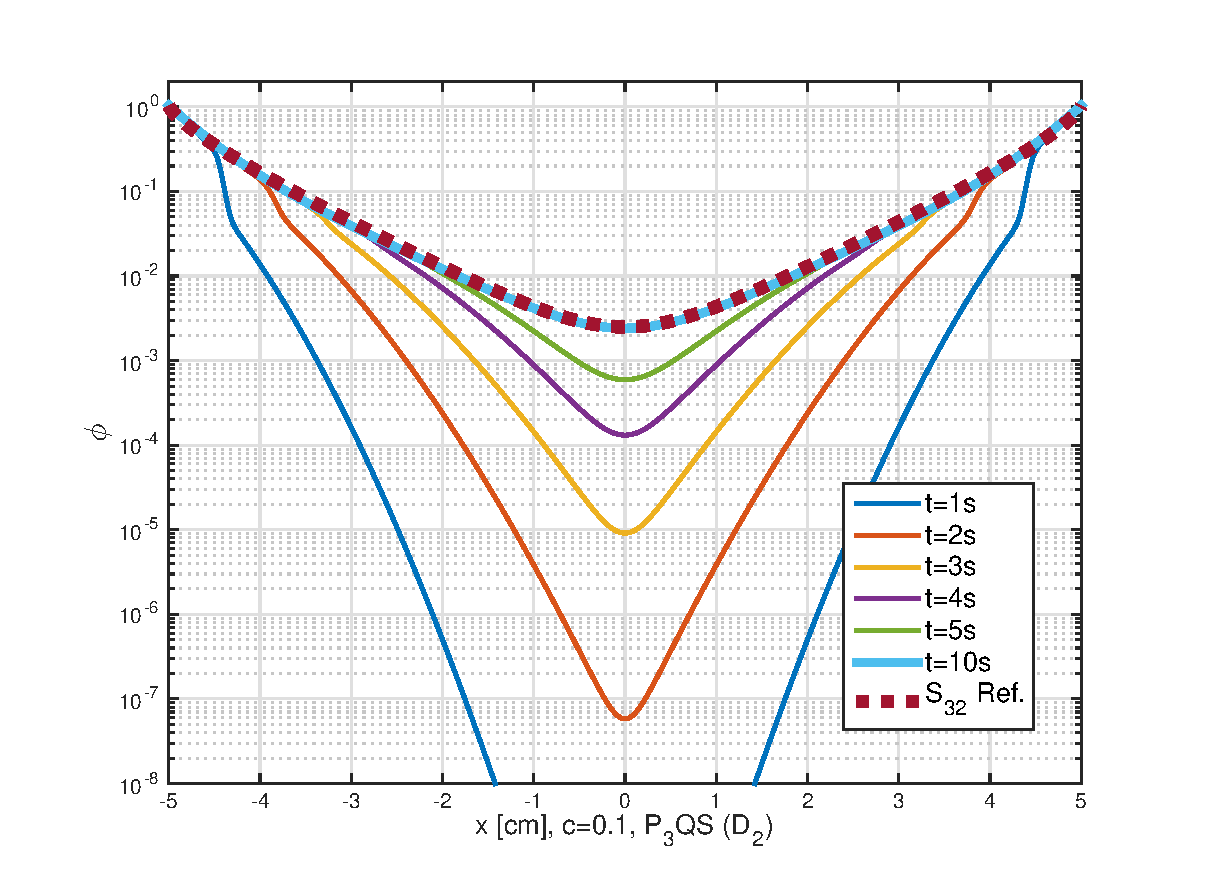
\includegraphics[width=1\linewidth]{brunner_p3qs.eps}
		%\caption{P$_3$QS (D$_2$) time-dependent solution}
		%\label{gptrhort}
	\end{subfigure}
	\caption{Comparison between P$_3$QT and P$_3$QS (D$_2$)~solutions to double incident problem.}
	\label{exp}
\end{figure}

\textcolor{red}{I shall talk about the method fixes the wavefront. Also, the boundary treatment is on the list}
The second test problem is a highly absorbing problem with isotropic incident angular fluxes on both sides of a slab. The scattering ratio, $c$,~of the medium is $0.1$. The original test problem is in steady state. However, if one turns on the boundary flux at the beginning, eventually an accurate approximation to transport is supposed to present a similar result for the transport solution in steady state.

Though the incident flux is isotropic on the boundary, the angular flux gradually turns to become strongly anisotropic and form beam-like distribution in the middle of the slab due to the strong absorption. This beam-like behavior of the angular flux seems to be a potential challenge for the model. For some closure models, such as the entropy based closure model (M$_N$),~have difficulty in resolving the beam. For M$_N$~method, it tends to have artificial shock in the middle (Ref.~\cite{brunnerentropy,coryentropy}).~It is also suspected in Ref.~\cite{coryentropy}~that this shock could possibly caused by small errors when solving minimization problem governing the M$_N$~method. Fortunately, the flux limited closure does not have the artificial flux shock.
\subsubsection*{Limiter effects on wavefront}
Basically discuss Figure~\ref{exp}.

The P$_N$QT model, having a similar form as P$_N$QS (or D$_N$)~model, automatically adjusts the effective diffusion coefficient for the closed moment. Since the simulation in the double-incident problem is performed in a time-dependent way, a physical solution should preserve the property that before $t=L/(2v)$,~fluxes propagated from different incidents, shall not contact each other because the particle should not have a speed over $v$.

However, as shown in Figure~\ref{exp},~P$_3$QS (D$_2$)~over diffuses the particles such that the fluxes from different sides get contacted, which is like artificially accelerating the particles. Compared with this diffusive closure model, P$_3$QT, yet, somehow, limits the accelerations, which preserves very sharp wavefront.
%\begin{figure}[ht!]
%\centering
%\subfigure[P$_3$QT]{0.5\textwidth}
%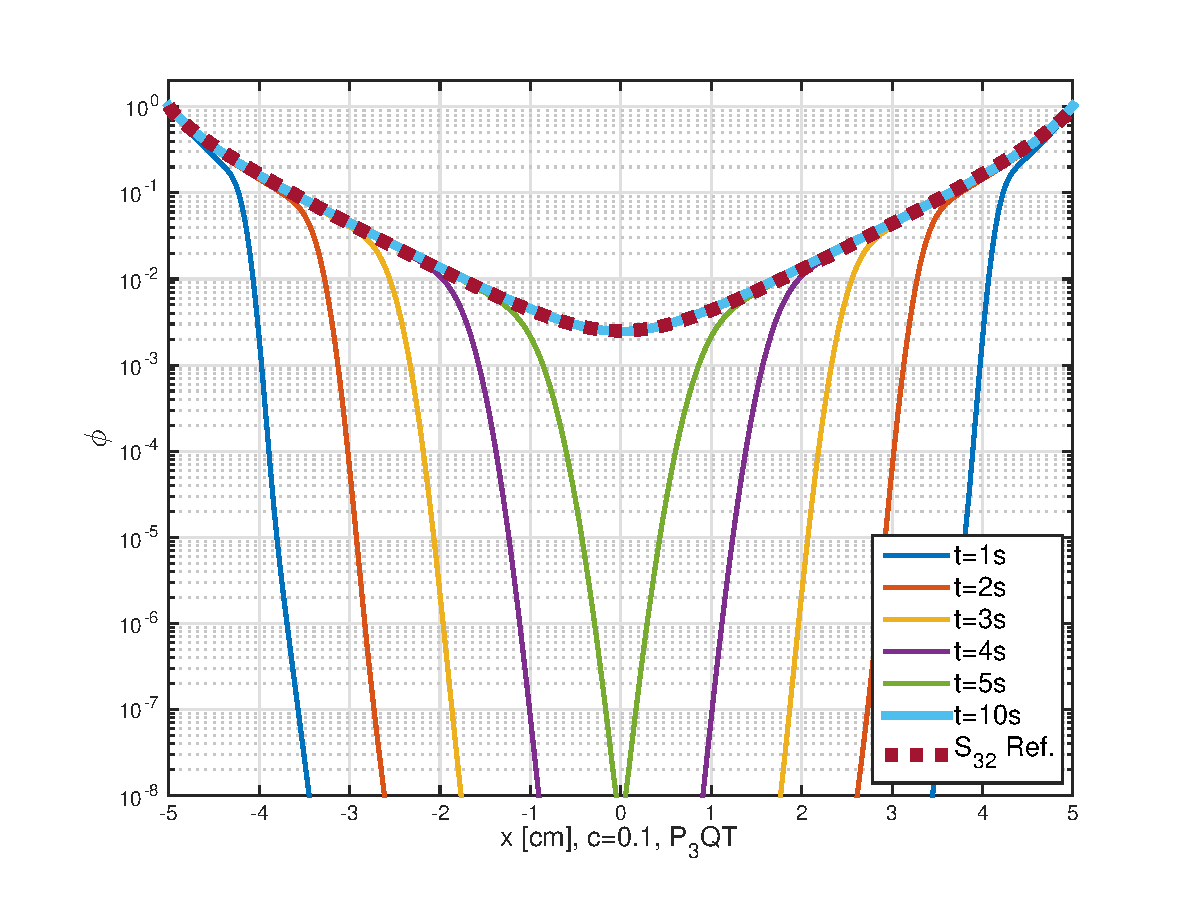
\includegraphics[width=0.9\linewidth]{brunner_p3qt.eps}
%\caption{Parameter significances (mean sums of squares) from ANOVA analysis.}
%\label{fg:anova_sig}
%\end{subfigure}
%~
%\begin{subfigure}{0.5\textwidth}
%\centering
%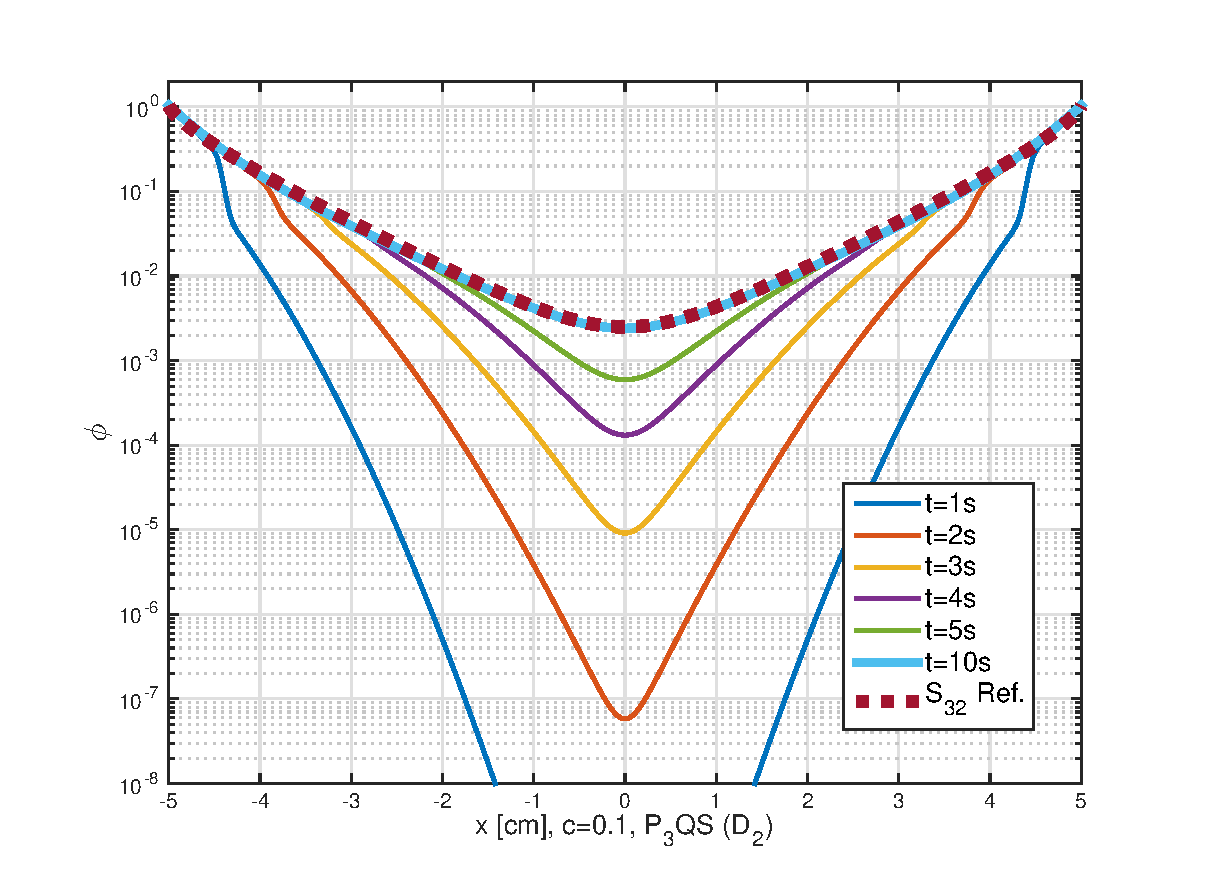
\includegraphics[width=0.9\linewidth]{brunner_p3qs.eps}
%\caption{Parameter significances (relative relevance) from GPR emulation.}
%\label{fg:gpr_sig}
%\end{subfigure}
%\caption{Parameter significance comparisons from different methods.}
%\label{fg:sigs}
%\end{figure}



%\begin{figure}[ht]
%\centering
%\begin{minipage}[b]{0.5\linewidth}
%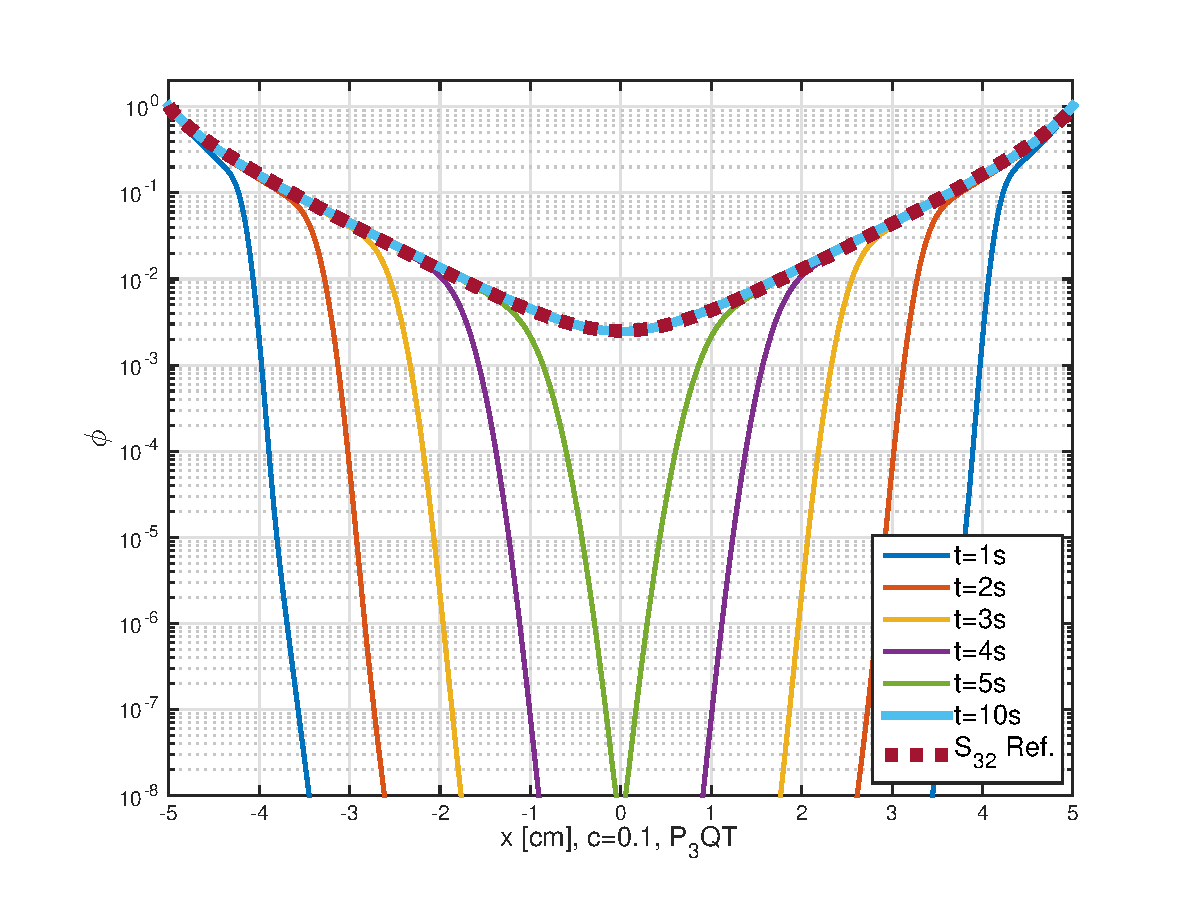
\includegraphics[width=0.19\linewidth]{brunner_p3qt.eps}
%\caption{Happy Smiley}
%\label{fig:minipage1}
%\end{minipage}
%\begin{minipage}[b]{0.5\linewidth}
%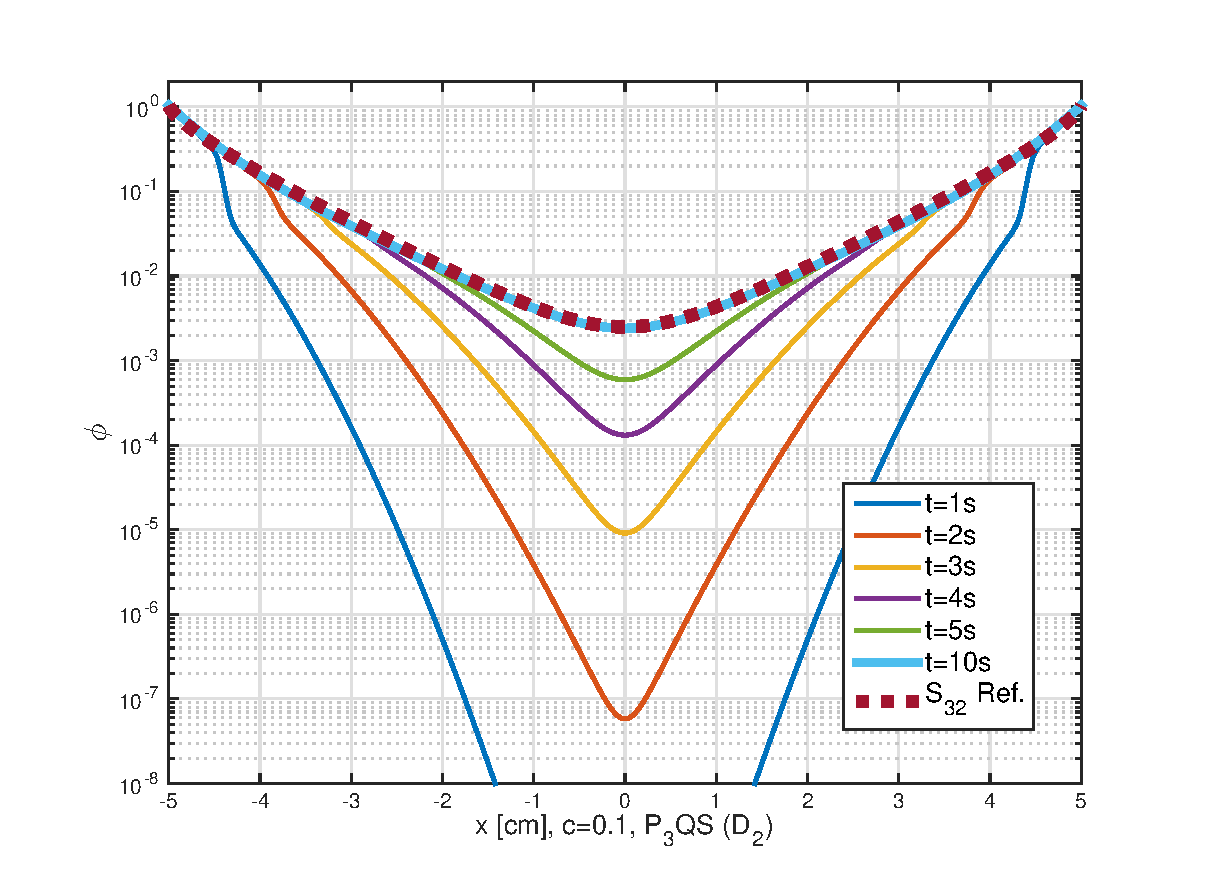
\includegraphics[width=0.19\linewidth]{brunner_p3qs.eps}
%\caption{Sad Smiley}
%\label{fig:minipage2}
%\end{minipage}
%\end{figure}


%\subsubsection*{Boundary condition test}

\subsection{Reed's problem: void treatment and material discontinuity}
The last test problem in this work is the Reed's problem. The configuration can be found in Ref.~\cite{reed_1971}. It contains several regions with largely varied properties including strong pure absorbers, voids, strong source and material discontinuities.

The numerical example in Figure~\ref{reed}~is the P$_5$QT solution of Reed's problem in time-dependent manner by turning on the source at $t=0$.~The aim is to test the model accuracy on facing such a senario with large material changes. Moreover, since the developing closure is similar as a Fick's law, the behaviour of the model in voids is also of interest. 

Graphically, P$_5$QT agrees well with S$_{32}$~reference calculations, which is spatially discretized using DD with $2\times10^4$~cells. The strategy adapting P$_N$QT model to working in voids is via treating the cross section as:
\begin{equation}
\bar{\st}=\st+\zeta\delta_{\st,0},
\end{equation}
where $\delta$~is the Kronecker function and $\zeta$~is a small number, which is fixed at $10^{-3}$~in this paper. Though there is no principle for choosing $\zeta$, it accomplished the goal.

\begin{figure}[ht!]
	\begin{center}
		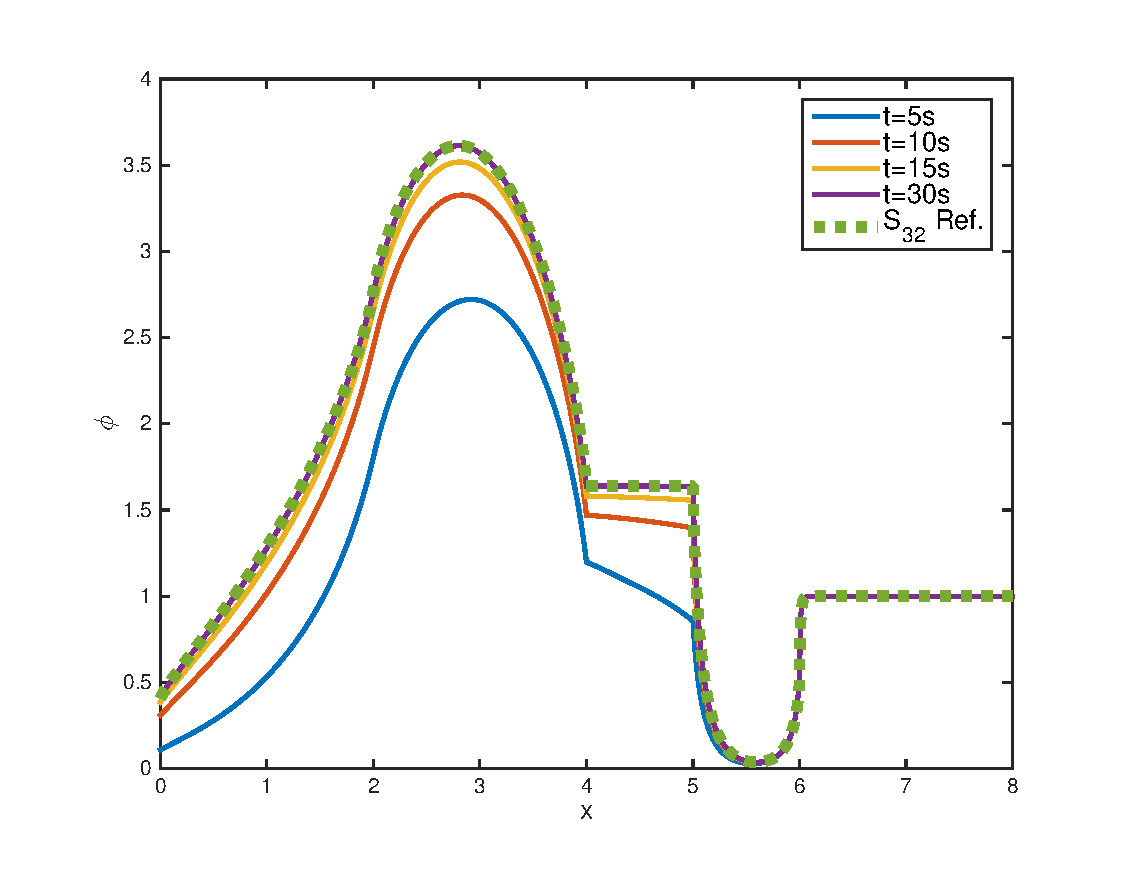
\includegraphics[width=1.\textwidth]{reed_p5qt.eps}
		%\includegraphics[width=0.45\textwidth]{srholam.eps}
		\caption[]{\label{reed}Reed problem solved with P$_5$QT.}% Only the ``Figure" label and figure number are bold.}
	\end{center}
\end{figure}

\section{Concluding remarks}
%\subsection{Summary}
In this paper, we novelly analyzed the effects on \pn~approximation residual with different closures. We provide a new explanation why conventional \pn~and \pn~with diffusive closure is inferior in transient simulations. Based on the analysis, we proposed two closures, the ``moment-limited" and ``flux-limited" closures and name them P$_N$~quasi transient models (\pnqt)~due to the fact that the models outperforms the \pn~and \pnqs~approximations.

%\subsection{Future work}
We believe P$_N$QT is a promising model motivating us extending the model to 2D with expecting accurate results as well in simulating particle transport. Also, in order to obtain high resolution with DD, we set very fine mesh with small time steps, which is impractical for large system and multi-D applications. A more decent discretization, e.g.~discontinuous Galerkin, shall be implemented.

Moreover, we see a hope that modifying the diffusive closure with flux limiters would generally bring high accuracy. It could then be worth investigating the behaviors of various flux limiters introduced in flux limited diffusion theories.

\section*{Acknowledgements}
Many thanks go to Dr. Jim E. Morel for critizing the idea of analyzing the residual. Also, I am grateful to Dr. Robert B. Lowrie's discussion to make the reasoning in theoretical part reasonable.


\section*{References}
\bibliography{mybibfile}

\end{document}